\documentclass[11pt]{article}
\usepackage[utf8]{inputenc}
\usepackage{graphicx}
\usepackage{enumitem}
\usepackage[margin=0.3in]{geometry}
\usepackage[dvipsnames]{xcolor}
\usepackage{yfonts}

\usepackage{aurical}
\usepackage[T1]{fontenc}
\usepackage{tabularx}
\usepackage{background}
\usepackage{MnSymbol}
\usepackage{tikz}
\newcommand*\circled[1]{\tikz[baseline=(char.base)]{
            \node[shape=circle,draw,inner sep=2pt] (char) {#1};}}
\definecolor{OCRA}{RGB}{204,119,34}
% Hit Points
\newcommand\MaxHitPoints{12}
\newcommand\CurrentHitPoints{5}
% Levels
\newcommand\FighterLevel{2}
\newcommand\MagicUserLevel{2}
% Spells
\newcommand\SpellSlotsLevelOne{2}
\newcommand\LevelOneSpellOne{Sleep}
\newcommand\LevelOneSpellTwo{Charm Person}
% Scrolls
\newcommand\ScrollOne{Web}
\newcommand\ScrollTwo{Mirror Image}
\newcommand\ScrollThree{Read Magic}
% removed color spray as it was used
\newcommand\ScrollFour{}
% Gear
\newcommand\EquipmentOne{Rope}
\newcommand\EquipmentTwo{Grappling Hook}
\newcommand\EquipmentThree{10 Pitons}
\newcommand\EquipmentFour{Hammer}
\newcommand\EquipmentFive{12 Torches}
\newcommand\EquipmentSix{}
\newcommand\EquipmentSeven{}
\newcommand\EquipmentEight{}
\newcommand\EquipmentNine{}



\begin{document}
\backgroundsetup{           % I insert it in the "title_page.tex" file
 scale=1,
 angle=0,
 opacity=.8,  %% adjust
 contents={
\includegraphics[width=\paperwidth,height=\paperheight]{img/paper.jpg}}
 }
\begin{minipage}{0.4\textwidth}
    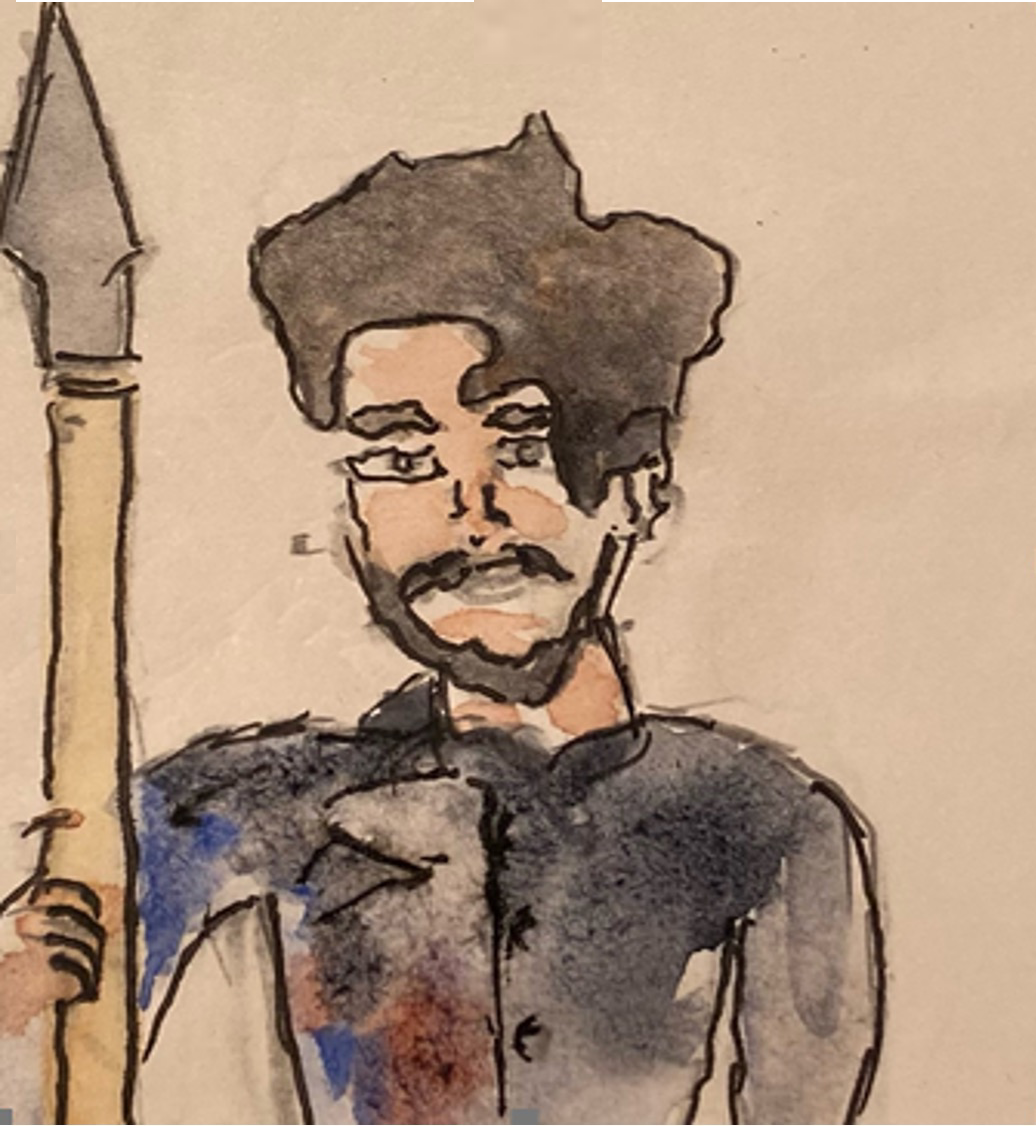
\includegraphics[scale=0.45]{img/arnosto.png}
\end{minipage}%
\hspace{0.4cm}
\begin{minipage}{0.55\textwidth}%\raggedleft
    \Huge{\Fontauri The Real Arnosto} \\
    \Large{Fighter \FighterLevel/Magic User \MagicUserLevel} \\
    \begin{normalsize}
        \begin{itemize}[topsep=0pt, itemsep=0pt, partopsep=0pt, parsep=0pt, leftmargin=*]
            \item Is about 5’ tall has bushy black hair has a beard that keeps growing back, no matter how often he shaves
            \item has bare feet, which is not uncommon in these parts
            \item has hazel eyes
            \item sports a minimal smile, in fact it is probably a quarter of a smirk; the only way to tell if he is happy is if you can see a sparkle in his eyes
        \end{itemize}
    \end{normalsize}
    \begin{large}
        \vspace{0.4cm}
        \begin{tabular}{cccccc}
            Str & Int & Wis & Dex & Con & Cha \\ \hline
            13 & 11 & 8 & 11 & 11 & 10\\ 
            $\ostar$ & & & & & 
        \end{tabular}
    \end{large}
    \vspace{0.4cm}

    \begin{minipage}[t]{0.2\textwidth}
        \begin{large}
            \begin{tabular}[t]{lc}
                \textcolor{OCRA}{Max HP} & \circled{\MaxHitPoints}\\
                \textcolor{OCRA}{Current HP} & \circled{\ \CurrentHitPoints}
            \end{tabular}
        \end{large}
    \end{minipage}
    \hspace{1.0cm}
    \begin{minipage}[t]{0.2\textwidth}
        \begin{large}
            \begin{tabular}[t]{lc}
                \textcolor{OCRA}{AC Leather} & \circled{\ 7}\\
                \textcolor{OCRA}{AC Mail} & \circled{\ 5}                
            \end{tabular}
        \end{large}
    \end{minipage}
    \hspace{1.0cm}
    \begin{minipage}[t]{0.2\textwidth}
        \begin{large}
            \begin{tabular}[t]{lc}
                \textcolor{OCRA}{AC Plate} & \circled{\ 3}\\
                \textcolor{OCRA}{Shield} & \circled{-1}
            \end{tabular}
        \end{large}
    \end{minipage}
\end{minipage}
\vspace{0.5cm}

By trade I am a weaver; I travel from keep to keep and every village between. Somewhere along the way I must have been infected (maybe bit?) but I just don’t know how or where. What I do know is that I felt strange on a stop at Ten Keep and someone suggested that I go see Señor Hopi to find out if he could help me. By the time I got to his place in the back corner of the keep I was sweating profusely and I felt as if my skin was on fire. I must have looked horrible as Señor Hopi was very alarmed when he saw me. What happened next I can tell you only based on what Señor Hopi told me as I was no longer aware of what was happening. I will tell you the story using Señor Hopi’s words:

\begin{quote}
    Your eyes were glowing as if on fire, this was not a fire of the natural type. I was certain that you were afflicted by Lycanthropy and I raced toward my altar in the hope that I could get to my scroll case and either save you or save myself. I was not sure which of us would still be breathing in the near future. You were tearing at your appendages and chest as if you were in horrible pain, which makes sense as your body was changing in horrible ways. I got to the scroll case and took a deep breath to calm myself, and started on the work to stop what was happening. As I finished reading the scroll you must have decided that I needed to die, or maybe the wolf in you made that decision, I hope that it was the wolf and not you. You came at me and used all of your strength to break through the stone altar between us. I finished the reading of the scroll just in time and you fell to the floor writhing in pain, it must have been horrible for you to change twice in just a few minutes as you slept for a day and a half. It was not a pleasant sleep.
\end{quote}

When I awoke I ached all over. I looked in the mirror and asked Hopi how long I had slept, from the length of my beard it must have been a week. Hopi smiled and said only two days. This was one of many surprises since then. Hopi told me that while I was asleep Rosa and Rueño helped keep watch over me and kept me tied to the bed.\\

In the months since there have been three full moons, including last night. My reaction has varied. The first two I slept in the back of one of our wagons (we had three that we travelled from place to place in, and one of them was fitted with an iron cage that Hopi strongly recommended that we built. The First People of La Tetrada did not understand why they were building an iron cage in the back of the wagon, but they had done odd jobs for Hopi in the past and did so again.
Last night there was no iron cage, and in fact I was not aware of the full moon until I awoke feeling strange. It was about midnight and we (Honey Badger, Anoki, and I) were all at the camp North of Depico’s place just outside of the Necromancer’s cave. When I realized that I was being affected by the moon I decided to leave camp to hunt and to get away from the party. I wanted to head for higher ground; did I need to be closer to the moon, or just away from my comrades? I went down the road to the west planning to head uphill. I took only a dagger and myself, with the full moon and my enhanced vision I did not need or want anything else. I made my way to the top of the hill and looked around. To the NorthWest I could see a very old road, I would like to believe that this leads to the tower that we can see on Rosa’s map. To the NorthEast I can see the lights of a village. Between here and there I can see the smaller lights of the wild creatures that we came across on a recent night (Cindershams), I do not want to meet them tonight.

\newpage

Closer to me I spot a few Antelope. I am hungry, and in a few days we will be out of rations unless we head back to Depico’s, so I hunt tonight. My dagger is between my teeth and I am staying as low to the ground as possible and moving quietly toward the Antelope. I think they are about 160 yards away, to far for a dagger or a spell. When I get half way to them I see their ears start to twitch, if they run I will also, but I would rather take them here and not out by the Cindershams. I don’t want to use a spell, but I don’t want to go hungry either, so I grab some sand and toss it in the air as I cast a sleep spell. The Antelope fall and I race forward. I grab one and carefully slit it’s throat and put it aside. The rest I kick to awaken them and they scatter. I head back uphill with the single Antelope and make my way back to camp where I join my friends and rest.

\vspace{1.4cm}
\begin{minipage}[t]{.5\textwidth}
{\huge \Fontauri Features}\\
\textcolor{OCRA}{Kenku}\\
\textbf{Mimica} Puoi riprodurre i suoni che hai sentito, incluse le voci.\\
\textbf{Contraffazione Esperta} Puoi duplicare manufatti e scritture di altre creature. Disponi di vantaggio \\
\textcolor{OCRA}{Bard}\\
\textbf{Bardic Inspiration}(d8)\\
\textbf{Jack of all trades} Half Proficiency to Ability Check\\
\textbf{Song of Rest} 1d6 to Short Rest\\
\textbf{Font of ispiration} BI regained with Short Rest\\
\textbf{Countercharm} As an action start to sing. All allies in 30f have adv on being charmed or frightened.\\
\textcolor{OCRA}{College of Lore}\\
\textbf{Cutting Words} When a creatures make an attack roll 60f from you you can use a BI and sub from the attack.\\
\textbf{Additional Magic Secrets}\\
\textcolor{OCRA}{Rouge}\\
\textbf{Cunning Action}\\
\textbf{Sneak Attack (1d6)}\\
\end{minipage}
\begin{minipage}[t]{.4\textwidth}\raggedleft
\begin{center}
{\Huge \textgoth{P}} \circled{\Huge +4} \hspace{0.3cm} {\Huge \textgoth{A}} \circled{\Huge+8} \hspace{0.3cm} {\Huge \textgoth{S}} \circled{\Huge+9} {\Huge \textgoth{Q}} \circled{\Huge+2}
\end{center}

\vspace{0.5cm}
{\Large \textbf{\Fontauri Skills}}\\
Athletics $\bullet$\\
Acrobatics \\ 
Deception $\bullet$\\ 
Investigation \\
Perception $\bullet$ \\
Performance $\bullet$\\ 
Stealth $\bullet$ \\

\vspace{.5cm}

{\Large \textbf{\Fontauri Sailor Background}}\\
A belaying pin(club)\\
50 feet of silk rope\\
A gemstone (coal for others)\\

\vspace{0.5cm}

{\Large \textbf{ \Fontauri Tools}}\\
Navigator's tools\\
vehicle(water)\\


\end{minipage}

\newpage

\begin{minipage}[t]{.25\textwidth}
{\huge \textbf{\Fontauri Spells}}\\
\textcolor{OCRA}{Level 1 slots: \SpellSlotsLevelOne }\\
\LevelOneSpellOne\\
\LevelOneSpellTwo
\end{minipage}
%\hspace{1.5cm}
\begin{minipage}[t]{.25\textwidth}
{\huge \textbf{\Fontauri Scrolls}}\\
\ScrollOne\\
\ScrollTwo\\
\ScrollThree\\
\ScrollFour
\end{minipage}
%CONTINUE OF EQUIPMENT
\begin{minipage}[t]{.4\textwidth}%\raggedleft
{\huge \textbf{ \Fontauri Equipment}}\\
\EquipmentOne\\
\EquipmentTwo\\
\EquipmentThree\\
\EquipmentFour\\
\EquipmentFive\\
\EquipmentSix\\
\EquipmentSeven\\
\EquipmentEight\\
\EquipmentNine
\end{minipage}
\newpage
%\backgroundsetup{           % I insert it in the "title_page.tex" file
 %scale=1,
 %angle=0,
 %opacity=.1,  %% adjust
 %contents={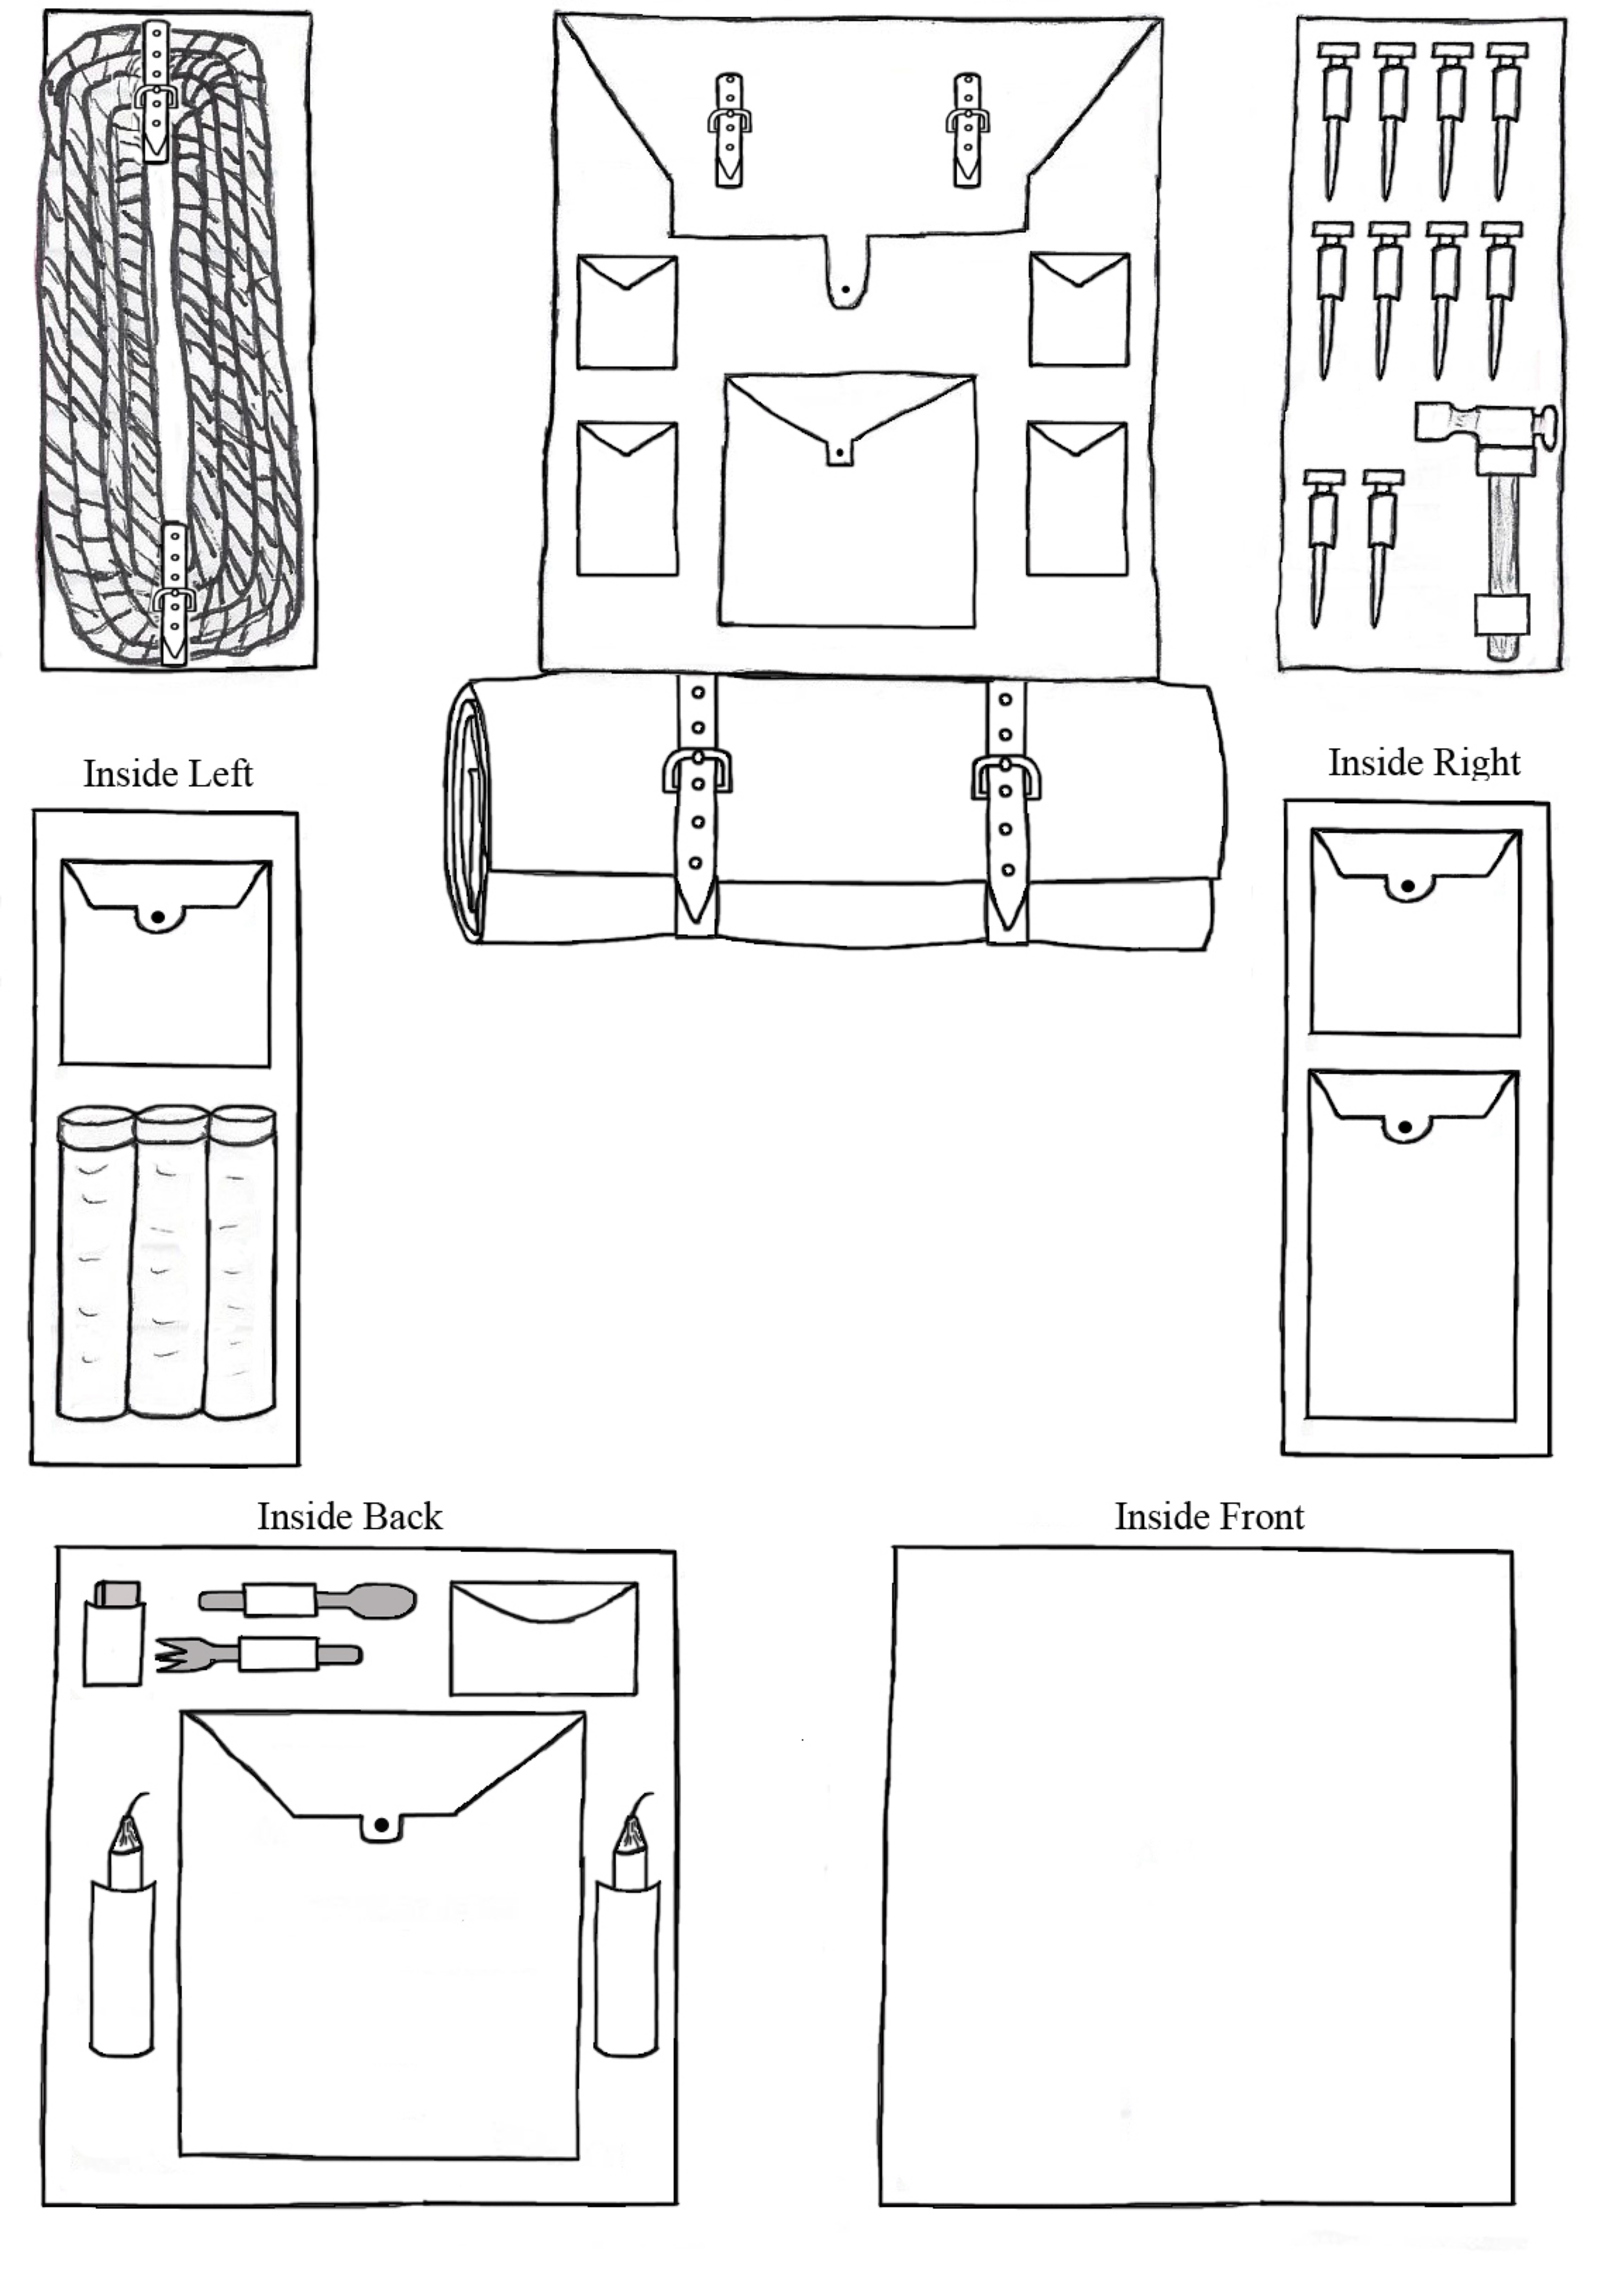
\includegraphics[width=\paperwidth,height=\paperheight]{img/backpack.jpg}}
 %}
Hello
\begin{minipage}[t]{0.2\textwidth}
\backgroundsetup{           % I insert it in the "title_page.tex" file
 scale=1,
 angle=0,
 opacity=.1,  %% adjust
 contents={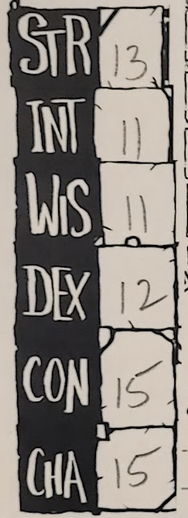
\includegraphics[width=\paperwidth,height=\paperheight]{img/saving.jpg}}
 }
 42
\end{minipage}
\end{document}
